% Options for packages loaded elsewhere
\PassOptionsToPackage{unicode}{hyperref}
\PassOptionsToPackage{hyphens}{url}
%
\documentclass[
]{article}
\usepackage{amsmath,amssymb}
\usepackage{lmodern}
\usepackage{iftex}
\ifPDFTeX
  \usepackage[T1]{fontenc}
  \usepackage[utf8]{inputenc}
  \usepackage{textcomp} % provide euro and other symbols
\else % if luatex or xetex
  \usepackage{unicode-math}
  \defaultfontfeatures{Scale=MatchLowercase}
  \defaultfontfeatures[\rmfamily]{Ligatures=TeX,Scale=1}
\fi
% Use upquote if available, for straight quotes in verbatim environments
\IfFileExists{upquote.sty}{\usepackage{upquote}}{}
\IfFileExists{microtype.sty}{% use microtype if available
  \usepackage[]{microtype}
  \UseMicrotypeSet[protrusion]{basicmath} % disable protrusion for tt fonts
}{}
\makeatletter
\@ifundefined{KOMAClassName}{% if non-KOMA class
  \IfFileExists{parskip.sty}{%
    \usepackage{parskip}
  }{% else
    \setlength{\parindent}{0pt}
    \setlength{\parskip}{6pt plus 2pt minus 1pt}}
}{% if KOMA class
  \KOMAoptions{parskip=half}}
\makeatother
\usepackage{xcolor}
\usepackage[margin=1in]{geometry}
\usepackage{longtable,booktabs,array}
\usepackage{calc} % for calculating minipage widths
% Correct order of tables after \paragraph or \subparagraph
\usepackage{etoolbox}
\makeatletter
\patchcmd\longtable{\par}{\if@noskipsec\mbox{}\fi\par}{}{}
\makeatother
% Allow footnotes in longtable head/foot
\IfFileExists{footnotehyper.sty}{\usepackage{footnotehyper}}{\usepackage{footnote}}
\makesavenoteenv{longtable}
\usepackage{graphicx}
\makeatletter
\def\maxwidth{\ifdim\Gin@nat@width>\linewidth\linewidth\else\Gin@nat@width\fi}
\def\maxheight{\ifdim\Gin@nat@height>\textheight\textheight\else\Gin@nat@height\fi}
\makeatother
% Scale images if necessary, so that they will not overflow the page
% margins by default, and it is still possible to overwrite the defaults
% using explicit options in \includegraphics[width, height, ...]{}
\setkeys{Gin}{width=\maxwidth,height=\maxheight,keepaspectratio}
% Set default figure placement to htbp
\makeatletter
\def\fps@figure{htbp}
\makeatother
\setlength{\emergencystretch}{3em} % prevent overfull lines
\providecommand{\tightlist}{%
  \setlength{\itemsep}{0pt}\setlength{\parskip}{0pt}}
\setcounter{secnumdepth}{-\maxdimen} % remove section numbering
\usepackage{float}
\floatplacement{figure}{H}
\ifLuaTeX
  \usepackage{selnolig}  % disable illegal ligatures
\fi
\IfFileExists{bookmark.sty}{\usepackage{bookmark}}{\usepackage{hyperref}}
\IfFileExists{xurl.sty}{\usepackage{xurl}}{} % add URL line breaks if available
\urlstyle{same} % disable monospaced font for URLs
\hypersetup{
  pdftitle={STA304 - Fall 2022},
  pdfauthor={Eric Zhu - 1005131368},
  hidelinks,
  pdfcreator={LaTeX via pandoc}}

\title{STA304 - Fall 2022}
\usepackage{etoolbox}
\makeatletter
\providecommand{\subtitle}[1]{% add subtitle to \maketitle
  \apptocmd{\@title}{\par {\large #1 \par}}{}{}
}
\makeatother
\subtitle{Assignment 1}
\author{Eric Zhu - 1005131368}
\date{30/09/2022}

\begin{document}
\maketitle

\hypertarget{part-1}{%
\section{Part 1}\label{part-1}}

\hypertarget{goal}{%
\subsubsection{Goal}\label{goal}}

A Graphics Processing Unit is a microprocessor that is suited for
certain kinds of computations. Fundamentally, a GPU is a SIMD device
(simultaneous instruction multiple data) device that enables much faster
computation of matrix heavy operations, e.g., computer graphics and
certain kinds of numerical optimization algorithms (gradient descent).
They were originally built to accelerate rasterization performance
(image rendering) across computer rendering with GPU cores that
performed much faster than CPU cores for rendering thanks to task
specialization {[}3{]}. Regardless of their origins, traditional GPU
cores have been fundamental to machine learning experimentation,
scientific modelling, and entertainment.

In recent years, GPUs have gotten more capabilities via specialized
hardware for tasks like real-time ray tracing (simulating realistic
lighting) and half-precision (16 bit) matrix math {[}1{]}. Consumers
have found this to be of dubious value depending on their background and
use cases, leading to discussions across the industry and community
about what functions GPUs should prioritize {[}2{]}. As the GPU market
continues its strong growth, slated to become a 200.85 billion dollar
market by 2027 {[}4{]}, the question over GPU functionality preferences
also grows in importance and relevance. While there may be many
preferences for GPU capabilities, the preferences we wish to focus on
are based on the distinct hardware capabilities that are most relevant
across consumer categories, i.e., traditional GPU cores for
rasterization/compute capabilities, real-time ray-tracing hardware, and
hardware for half-precision matrix math (will also be referred to as
half precision hardware). Essentially, we are aiming to examine the
question: what kind of GPU user wants what kind of GPU hardware?

\hypertarget{procedure}{%
\subsubsection{Procedure}\label{procedure}}

Fundamentally, our goal is to analyse the preferences of GPUs across the
consumer categories, including a diverse set of users with wildly
different use cases. Thus, our target population is simply the users of
GPUs across these different categories, and specifically for this
survey, we are looking at two aggregated categories (professionals and
consumers). The frame population is dependent on the likely ways of
distributing this survey. The easiest way of distributing this survey
would be through online forums of GPU users. Other ways would have
significant drawbacks. For example, distributing it through exit surveys
after GPU purchasing would leave us a biased same from those who use
GPUs but do not directly purchase or install them, e.g., academics who
run experiments on GPUs. Or the other option of using customer data
collected by ``game optimization'' software from the manufacturer (like
GeForce Experience) would bias our sample given that it is generally
uncommon for enterprise settings to install these apps (e.g., AWS does
not install these) and would potentially lead to biases for certain GPU
manufacturers. Since forums are targeted to a specific demographic, it
would make the most sense for us to employ stratified random sampling as
this strategy follows most naturally from targeted forums where we would
distribute our survey as they naturally form self-selecting strata. This
is advantageous over other sampling methods, namely cluster random
sampling. This is because it is simply unfeasible to form representative
clusters with online forums, i.e., forum membership is voluntary and
forum topic is predetermined. In other words, there is no good way of
getting lists of users from forums like Reddit where such information is
private. Thus the only feasible way would be to scrape users who comment
and post as those are the only two publicly available pieces of user
information. Then we'd have to send those users messages about our
survey (after forming clusters), which could introduce bias should we
use them as our sample since users who post generally are more vocal or
passionate about some subject. So cluster random sampling could
introduce worrying sources of sample bias. While stratified random
sampling is definitely the better option among others, the major
downside is that members of certain strata may belong in many strata,
e.g., it is reasonable to assume that there are overlaps between gamers
and academics (perhaps some PhD student plays video games). This may
introduce some sampling bias as we might over/under represent some
groups; this is unavoidable even with a different sampling technique as
this source of bias is inherent to the individual so this bias would
still be present regardless of sampling technique.

\hypertarget{showcasing-the-survey.}{%
\subsubsection{Showcasing the survey.}\label{showcasing-the-survey.}}

Survey link: \url{https://forms.office.com/r/uqb23eNtc7}

I chose the following three questions overall because the first two are
representative of questions that would enter the models as covariates,
while the third question would enter the model as a response variable.

\textbf{Question 1: Estimated hours per day of intensive GPU usage?
Intensive usage could be an application like training Deep Learning
models, running 3D graphics applications like games, and or rendering
videos.}

This question is meant to gather information measuring the participant's
familiarity of GPUs. The logic here is that the longer a user uses a GPU
for their specified use case (e.g., a deep learning researcher
interfacing with GPU based deep learning libraries), the more familiar
that user would be with GPUs and their capabilities. This is similar to
the logic how we could reasonably conclude that a person is familiar the
functionality of their laptop should they use it a lot. An inherent
drawback to this question is that it doesn't ask directly about a user's
perceived familiarity with GPUs (perhaps on some scale, e.g., 1 to 10),
so it's a proxy for it. But this is done because perceived familiarity
can be heavily biased by their own perception, so this provides a more
absolute measure of familiarity with GPUs. Another potential drawback is
that since we allow for any input, this question measures the estimated
minutes on a continuous scale; perhaps a discrete scale could provide us
with the ability to model this variable using random effects, but this
was done because there's no good cutoff for each group. In other words,
a cutoff would be misinformed and could possibly lead to skewed
analysis.

\textbf{Question 2: What type of GPU do you usually use?}

Options:

\begin{itemize}
\item
  Datacentre/HPC (Nvidia A series, AMD instinct)
\item
  High end consumer (Nvidia xx80 (ti), Nvidia xx90(ti), AMD x800,
  x800xt, x900xt, e.g., Nvidia RTX 3080)
\item
  Midrange consumer (Nvidia xx70 (ti), Nvidia xx60(ti), AMD x700,
  x700xt, x600xt, e.g., Nvidia RTX 3070)
\item
  Entry level consumer (Otherwise: Nvidia xx50 and below, AMD x500 and
  below, e.g., Nvidia RTX 3050)
\end{itemize}

This question is meant to gather information measuring the effect on GPU
capability preferences due to a user's hardware segmentation. In other
words, we are looking to gather information on if using a certain kind
of GPU would affect their preferences for GPU hardware capabilities
because different ``levels'' of GPUs have different characteristics. The
logic here is comparable to asking a car owner about their current car
in a survey about car feature preferences. Additionally, a strong point
is that the categorization of the options is based on industry
standards. As in, the datacentre/HPC categorization and corresponding
examples (Nvidia A series, AMD instinct) are based on how they are
marketed by both companies. For the consumer options (last 3), those are
based on search results/a listing from Best Buy, a major electronics
retailer {[}12{]} {[}13{]}. This should mean that there is very little
ambiguity (given our exhaustive options listing) for the survey taker in
choosing their appropriate category since this categorization would be
exactly the same categories GPU buyers are exposed to. The final major
pro of this question is that it is implicitly ordered, i.e., the
categories are ordered by price, so we could examine how different GPU
price categories affect preferences too. However, the downside to this
is that some users may not necessarily agree with these categories, so
they may not choose to follow the examples in the parenthesis as stated
in the four options.

\textbf{Question 3: How important are traditional GPU cores in GPUs?
Consider 50 to be neutral and 100 to be a strong like; negative scores
will indicate a strong dislike. Decimals are allowed. }

This question is meant to gather information on a user's preference for
traditional GPU cores, which is the response variable for one of the
models. This question is repeated three times for the three hardware
categories, i.e., traditional GPU cores, ray-tracing hardware, and
half-precision matrix math (half-precision) hardware. We allow for
decimal values so that it is appropriate later to model the response
with a continuous probability distribution. So this question is meant to
be interpreted along side the other two, and this is a major strength
over making the user choose a particular specialized hardware preference
or even a ranking. Primarily, this will allow us to examine all three
hardware categories independently should the same covariates affect the
response variable differently for each hardware category, i.e., we can
get separate effect size estimations for the same covariates but for
different response variables. A drawback is that this scale is not
rigorously defined, and is the most open ended question in the survey.
This is because GPU users may not consider the same scale as the other
users, e.g., \(50\) may be neutral to some users but may indicate a
slight preference to others. To remedy this I added the ``and 50 being
neutral'' part of the question. Nonetheless, users will likely still
consider the scale to be slightly different based on their own
experiences. A discrete scale, e.g., categories of preferences, could
have been better as it would be more rigorously defined (labeled
categories), but there would still be some bias regardless since the
source of bias is the individual's conception of the scale, i.e., how
they conceptualize favour for some hardware capability.

\newpage

\hypertarget{part-2}{%
\section{Part 2}\label{part-2}}

\hypertarget{data}{%
\subsection{Data}\label{data}}

We are looking to simulate the data due to practical sampling
constraints. We have a few main considerations: the demographics that we
are look to simulate, and the effects stemming from the covariates we
wish to measure. At a high level, we are looking to measure the
preferences of individuals, given their use cases, for the three kinds
of hardware in GPUs we are considering: GPU cores, ray-tracing hardware,
and half-precision matrix math hardware. Since it is conceivable that
certain variables from our survey, e.g., type of GPU user will affect
the preferences overall for a user type, we will consider the data
generation in a so-called hierarchical manner.

First, we need to simulate our target population, i.e., what are the
proportions of our GPU user types? While the number of each GPU user
type wouldn't be released as public information (think military users or
sensitive corporate situations like Amazon AWS), we can inform this
simulation choice using publicly available earnings data from the two
major GPU makers: Nvidia and AMD. In both cases, their public earnings
data show that they sell roughly equally to the consumer and
professional markets in Q1 of 2022 {[}5{]}{[}6{]}. Thus, we will first
sample from the Bernoulli distribution with a parameter \(p=0.5\), i.e.,
it is equally likely for us to choose a professional or a consumer GPU
user.

Second, with a user category chosen, we then need to simulate the next
three survey questions that will act as covariates in our model, i.e.,
factors that could affect GPU hardware category preferences. Recall that
the last 3 questions are essentially response variables that ask users
for their preferences of GPU hardware categories.

The second question in our survey asks the user their primary
interaction with their GPU. The question accepts three options:
programming libraries (like Pytorch), high level graphical interfaces
(like Photoshop), and graphics applications (like 3D games). The options
are implicitly ordered by ``invovledness'' of the user's primary
interaction with their GPU; in other words, we can provide an ordering
to the options based on how abstracted the user's primary interaction is
from dealing with the GPU. Since the ordering is based on how hands on
the user's primary interaction is, we have the ordering be that
programming libraries are the most hands on (a label of 3), followed by
graphics applications (a label of 2), then high level graphical
interfaces (a label of 1). In other words, programming libraries are
least abstracted and high level graphical interfaces are most abstracted
away from the GPU. Since we do not have access to how people use their
GPUs, we will have to come up with some sensible values for the
parameter of a categorical distribution to simulate this question.
Recall that a categorical distribution takes a vector of probabilities,
which in our case is dependent on the GPU user type (either professional
or consumer) and is of length 3. If our user is a professional, it is
sensible that the 60\% of professionals primarily interact with GPUs
through programming libraries (ML researchers, academics, software
engineers, etc\ldots), then 30\% of professionals interact with GPUs
through high level interfaces (creatives who use apps like Photoshop),
and then 10\% of professionals interact with GPUs through graphics
applications (video game designers and professionals who play a lot of
video games). Then for consumers, it is sensible that 80\% of consumers
interact with GPUs through graphics applications (primarily video games
as GPUs were initially made for them), then 10\% primarily use them for
programming libraries (those who may use them for ML personal projects),
and then 10\% primarily interact with them through high level graphical
interfaces (those who have them for editing photos or videos). So to
recap, we will simulate this variable by sampling from a
\(\texttt{Categorical}([0.6, 0.3, 0.1])\) distribution if they are a
professional and a \(\texttt{Categorical}([0.1, 0.1, 0.8])\)
distribution if they are a consumer.

The third question asks for the type of GPU the user uses. We
unfortunately do not have data from professionals about the distribution
of their GPU types since in many cases they may be custom or trade
secret information. However, from having used the University of Toronto
Computer Science department GPU clusters as part of projects in the
past, an institution like the University of Toronto uses almost
exclusively high end or datacentre class GPUs. The CS department website
also provides an example list of GPUs that are part of a general GPU
cluster at UofT {[}8{]}. With that in mind, we will simulate this
variable given a professional GPU user using the categorical
distribution where 50\% of professionals use datacentre GPUs, 40\% use
high end consumer models, 8\% use midrange consumer models, and 2\% use
low end consumer models. So provided a professional GPU user we sample
from \(\texttt{Categorical}([0.5, 0.4, 0.08, 0.02])\). Alternatively,
provided a consumer GPU user, we can look at the Steam hardware survey
to gather some insights. Steam is a major platform used for
buying/selling video games, accounting for 3.1 billion dollars in sales
for the first half of 2022 {[}9{]}. While these estimates are biased
towards gaming, it is the best large scale estimate of consumer GPU
types. Additionally, information is collected if the Steam user opts in;
it is not indicative of if the Steam user is primarily a gamer. From the
Steam hardware survey, we gather that essentially no consumer uses a
datacentre/HPC GPU, high end consumer GPUs account for approximately
10\% of consumer GPUs, and the rest is roughly evenly split between
midrange and entry level consumer GPUs. So given a consumer, we will
sample this variable from
\(\texttt{Categorical}([0, 0.1, 0.45, 0.45])\).

Then the fourth question asks about the estimated hours per week of GPU
usage. This variable, as mentioned previously, is a proxy for a user's
familiarity with GPUs as the longer they use a GPU through GPU based
tasks (like gaming) the more familiar they should be with GPUs. This is
also hard to simulate since a user's GPU usage is private information.
However, we can infer that it would be sensible that professional users
of GPUs use them for approximately 40 hours per week. So then, if we
were to generate samples for this variable, we could use a normal
distribution with a mean of 40 and a standard deviation of 5 (to account
for overtime or leaving early each work day). Then for consumers, we can
look to the ``The State of Online Gaming -- 2021 survey'', which
surveyed 4000 people in 8 countries. The survey was conducted by
Limelight, a cloud service provider. On average, they found that an
average gamer played 8 hours and 27 minutes of video games per week
{[}10{]}. Additionally, the top 25\% of gamers play more than 12 hours
per week. Using 12 hours per week as the \(75^{th}\) percentile (0.674
standard deviations from the mean), we can use the sample standard
deviation as the estimate for the population standard deviation, which
is \(\approx 5.2\) hours when solving for
\(0.674 \cdot \hat{\sigma}_{sample} = 3.5\) {[}10{]}. So then, if we
were to generate samples for this variable, we could use a normal
distribution with a mean of 9 and a standard deviation of 5.2. To recap,
given a professional user, we will sample from \(\mathcal{N}(40,~ 5)\),
and provided a consumer, we will sample from \(\mathcal{N}(9, ~5.2)\).
Finally, we will absolute all of the samples should there be a negative
sample as negative hours is nonsensical.

Finally, we will need to weight these simulated variables to compute a
conditional expectation for the three response variables. Then, we will
use this mean as the mean to a normal distribution. We will also use a
constant variance parameter (one \(\sigma^2\) for all \(x_i\)'s) because
we do not have data to allow us to faithfully make simulation choices
for different \(\sigma^2\).

As mentioned previously, we should model the GPU user type
hierarchically, meaning that we find it reasonable that the type of user
affects the baseline for GPU hardware category preference scores. We
will set both the professional and consumer baseline preference for
traditional GPU cores as 60 because they are used in almost all GPU
applications {[}3{]}. Then we will set the baseline preferences for
ray-tracing hardware as much higher in consumers than professionals as
that hardware is really only used in video games, so we will set the
baseline preference of consumers to 50 (neutral) and 10 for
professionals {[}2{]}. Finally, we set the baseline preferences for
half-precision matrix math hardware as both 55 for consumers and
professionals because they are used in AI task acceleration, which is
rapidly used more and more in both consumer applications (video game
upscaling {[}18{]}) and professional applications (deep learning
training {[}19{]}).

We will first consider the weights for the second survey question (a
user's primary interaction with their GPU). As mentioned previously, the
primary interaction questions are ranked in order from least interaction
to most interaction. Thus, we need to choose a weight for this question
that is sensical to interpret with respect to preference scores and
other levels. We choose 4 to be our weight because since we have 3
levels, the ``top'' level, i.e., programming libraries, would have a
total contribution of 16 to the total preference score, which is
reasonable. This is because the way a user interacts with their GPU
should be pretty informative for how perceive it. Additionally, we add a
negative constant of -2 to the baseline weight of 4 for consumer users
when it comes to ray tracing and half-precision hardware because those
pieces of hardware are more advanced, and consumer users, on average,
likely use them less.

Then we consider the weights for the third survey question (type of
GPU). Also recall that the options are ordered in terms of price for
these GPUs, so like the previous we need to choose a weight that is
sensical for the 4 levels we have, i.e, our top level will have a 4
times contribution to the final preference score over the baseline
level. We choose the weights to be 2 for the traditional GPU cores and
half-precision matrix math hardware categories, but 0.5 for the ray
tracing category. This is representative of the fact that ray-tracing
isn't nearly as important as tradition hardware currently. For ray
tracing hardware, we choose 0.5 since real-time ray tracing is still
rather niche {[}2{]}. We once again adjust these weights for consumers
because they have a different distribution of GPUs, owing to their use
case. So we choose weights for the traditional GPU cores and
half-precision matrix math hardware categories to be 1 each. This is
representative of consumer use cases, e.g., video games, where, across
the board, experiences are more curated relative to professionals.

Finally, we consider the weights for the fourth survey question (hours
of usage per week). We will weight this effect for all three categories
as 0.25 since each individual hour sensibly contributes very little to a
user's overall perception of GPU capabilities. Additionally, we find no
reason to suggest that a professional user's hour GPU use would be
weighted differently than a consumer's. Indeed, they use their GPUs
differently, but the usage is meaningful to both categories, which is
then reflected in their preference scores for different hardware.

Then the individual computed conditional expectations were used as the
mean for a normal distribution. Here we use a constant standard
deviation for all conditional expectations simply because there is no
data to otherwise inform a different modelling choice. We use a standard
deviation of 5 because this allows for some amount of variation, which
should represent individual variation due to sources like question
interpretation/interpretations of scale (how much dislike must a user
have to warrant a negative score) despite answering the same on survey
questions.

For this simulated dataset, we simulated 1000 conditional means using
the seed 123, then for each conditional mean, 10 samples were generated
from the parameterized normal distribution. So overall, there are 10000
samples in this simulated dataset.

\textbf{Note:} Since the data was simulated, there was no data cleaning
involved.

Below is a table of the important variables from our simulated dataset:

\begin{longtable}[]{@{}
  >{\raggedright\arraybackslash}p{(\columnwidth - 2\tabcolsep) * \real{0.3068}}
  >{\raggedright\arraybackslash}p{(\columnwidth - 2\tabcolsep) * \real{0.6932}}@{}}
\caption{The table of the important variables of simulated
dataset}\tabularnewline
\toprule()
\begin{minipage}[b]{\linewidth}\raggedright
Variable
\end{minipage} & \begin{minipage}[b]{\linewidth}\raggedright
Description
\end{minipage} \\
\midrule()
\endfirsthead
\toprule()
\begin{minipage}[b]{\linewidth}\raggedright
Variable
\end{minipage} & \begin{minipage}[b]{\linewidth}\raggedright
Description
\end{minipage} \\
\midrule()
\endhead
\texttt{user} & The binary encoded user type, i.e., professional (0) and
consumer (1) \\
\texttt{GPUType} & Integer encoded type of GPU (ordered by price), i.e.,
datacentre/HPC (4), high end consumer (3), midrange consumer (2), entry
level (1) \\
\texttt{primaryInteraction} & Integer encoded user's primary interaction
with a GPU (ordered by use case's abstraction from GPU) , i.e.,
programming libraries (3), graphics applications (2), high level
graphical \\
\texttt{weeklyHours} & The number of hours per week that the user uses
their GPU \\
\texttt{simulations.tradGPUCores} & The simulated preference for
traditional GPU cores ~given other simulated survey responses \\
\texttt{simulations.rayTraced} & The simulated preference for ray
tracing hardware ~given other simulated survey responses \\
\texttt{simulations.halfPrecision} & The simulated preference for half
precision matrix math ~hardware given other survey response \\
\bottomrule()
\end{longtable}

Below is the five number summary of the simulated traditional GPU cores
preference scores:

\begin{longtable}[]{@{}llllll@{}}
\caption{Five number summary of simulated traditional GPU cores
preference scores}\tabularnewline
\toprule()
Min. & 1st Quartile & Median & Mean & 3rd Quartile & Max \\
\midrule()
\endfirsthead
\toprule()
Min. & 1st Quartile & Median & Mean & 3rd Quartile & Max \\
\midrule()
\endhead
54.46 & 73.93 & 77.85 & 77.86 & 81.74 & 100.64 \\
\bottomrule()
\end{longtable}

Then, we have also have a five number summary of the simulated ray
tracing hardware preference scores:

\begin{longtable}[]{@{}
  >{\raggedright\arraybackslash}p{(\columnwidth - 10\tabcolsep) * \real{0.1343}}
  >{\raggedright\arraybackslash}p{(\columnwidth - 10\tabcolsep) * \real{0.2090}}
  >{\raggedright\arraybackslash}p{(\columnwidth - 10\tabcolsep) * \real{0.1493}}
  >{\raggedright\arraybackslash}p{(\columnwidth - 10\tabcolsep) * \real{0.1493}}
  >{\raggedright\arraybackslash}p{(\columnwidth - 10\tabcolsep) * \real{0.2090}}
  >{\raggedright\arraybackslash}p{(\columnwidth - 10\tabcolsep) * \real{0.1493}}@{}}
\caption{Five number summary of simulated ray tracing hardware
preference scores}\tabularnewline
\toprule()
\begin{minipage}[b]{\linewidth}\raggedright
Min.
\end{minipage} & \begin{minipage}[b]{\linewidth}\raggedright
1st Quartile
\end{minipage} & \begin{minipage}[b]{\linewidth}\raggedright
Median
\end{minipage} & \begin{minipage}[b]{\linewidth}\raggedright
Mean
\end{minipage} & \begin{minipage}[b]{\linewidth}\raggedright
3rd Quartile
\end{minipage} & \begin{minipage}[b]{\linewidth}\raggedright
Max
\end{minipage} \\
\midrule()
\endfirsthead
\toprule()
\begin{minipage}[b]{\linewidth}\raggedright
Min.
\end{minipage} & \begin{minipage}[b]{\linewidth}\raggedright
1st Quartile
\end{minipage} & \begin{minipage}[b]{\linewidth}\raggedright
Median
\end{minipage} & \begin{minipage}[b]{\linewidth}\raggedright
Mean
\end{minipage} & \begin{minipage}[b]{\linewidth}\raggedright
3rd Quartile
\end{minipage} & \begin{minipage}[b]{\linewidth}\raggedright
Max
\end{minipage} \\
\midrule()
\endhead
8.379 & 26.481 & 39.663 & 42.828 & 59.269 & 78.321 \\
\bottomrule()
\end{longtable}

Finally, we have a five number summary of the simulated half precision
matrix math hardware scores:

\begin{longtable}[]{@{}llllll@{}}
\caption{Five number summary of simulated half precision hardware
preference scores}\tabularnewline
\toprule()
Min. & 1st Quartile & Median & Mean & 3rd Quartile & Max \\
\midrule()
\endfirsthead
\toprule()
Min. & 1st Quartile & Median & Mean & 3rd Quartile & Max \\
\midrule()
\endhead
46.91 & 65.19 & 69.87 & 70.20 & 75.01 & 95.80 \\
\bottomrule()
\end{longtable}

From the three five number summaries, we see that the distribution of
the simulated traditional GPU cores preference scores had the least
variation as indicated by the IQR, the simulated half precision matrix
math hardware preference scores has the second most variation, and
simulated ray tracing hardware preference scores had the least.
Similarly, simulated traditional GPU cores preference scores had the
highest measures of centre (median and mean), simulated ray tracing
hardware preference scores had the second most, and simulated half
precision matrix math hardware had the least.

\begin{figure}

{\centering 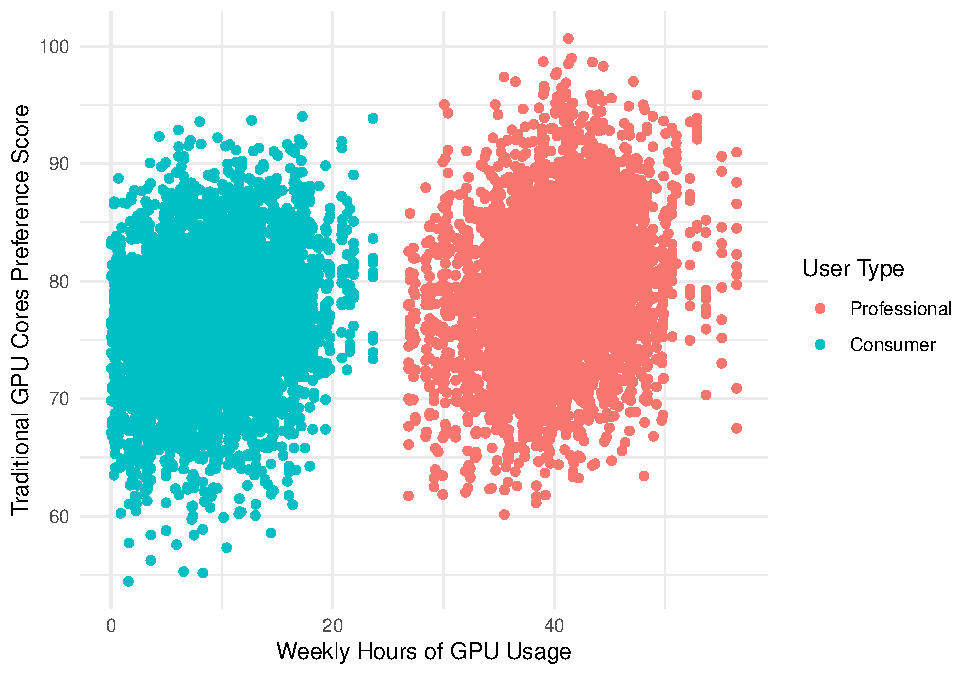
\includegraphics[width=0.6\linewidth,]{Assignment1_files/figure-latex/unnamed-chunk-6-1} 

}

\caption{Weekly Hours of GPU Usage vs Traditional GPU Cores Preference Score}\label{fig:unnamed-chunk-6}
\end{figure}

From the scatter plot of \texttt{Weekly\ Hours\ of\ GPU\ Usage} versus
\texttt{Traditional\ GPU\ Cores\ Preference\ Score}, we see that both
distributions are approximately Gaussian; however the consumer
distribution is not exactly Gaussian as weekly hours of GPU usage must
be greater than 0. Additionally, the Professional category of users has
a generally higher preference for traditional GPU cores. It appears that
the difference between the two user groups is just a shift up/down,
i.e., consumers appear to have been shifted down by some constant. The
spread between the distributions appear to be similar in general.

\begin{figure}

{\centering 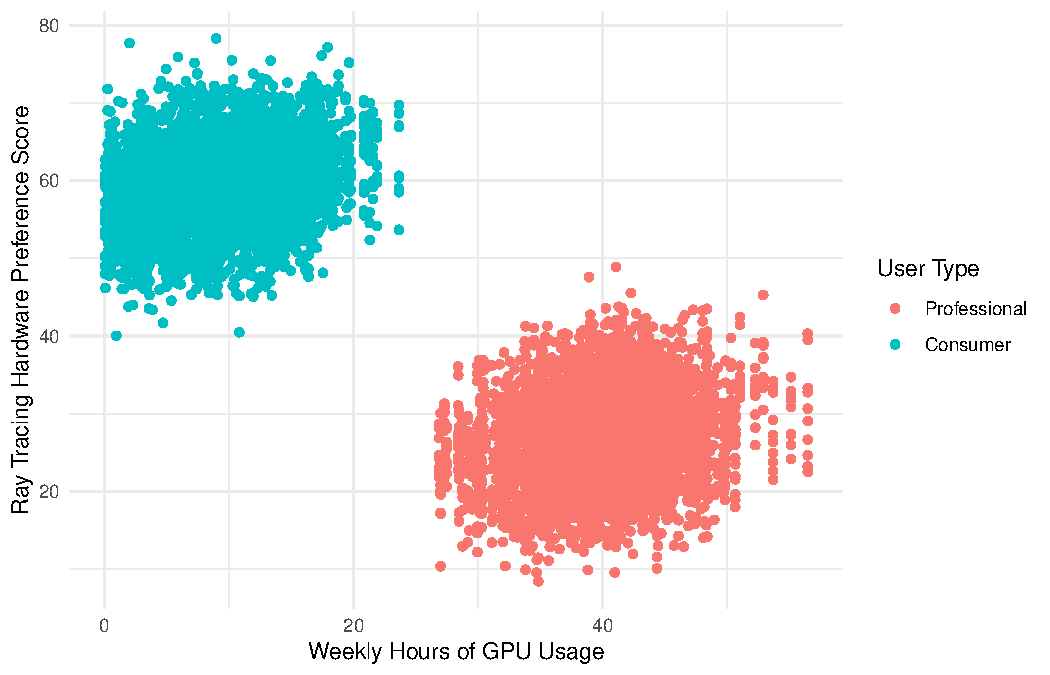
\includegraphics[width=0.6\linewidth,]{Assignment1_files/figure-latex/unnamed-chunk-7-1} 

}

\caption{Weekly Hours of GPU Usage vs Ray Tracing Hardware Preference Score}\label{fig:unnamed-chunk-7}
\end{figure}

From the scatter plot of \texttt{Weekly\ Hours\ of\ GPU\ Usage} versus
\texttt{Ray\ Tracing\ Hardware\ Preference\ Score}, we see that both
distributions are also approximately Gaussian; however the consumer
distribution is not exactly Gaussian as weekly hours of GPU usage must
be greater than 0. Additionally, the Consumer category of users has a
generally higher preference for ray tracing hardware. It appears that
the difference between the two user groups is just a shift up/down,
i.e., professionals appear to have been shifted down by some constant.
The spread between the distributions appear to be similar in general.

\begin{figure}

{\centering 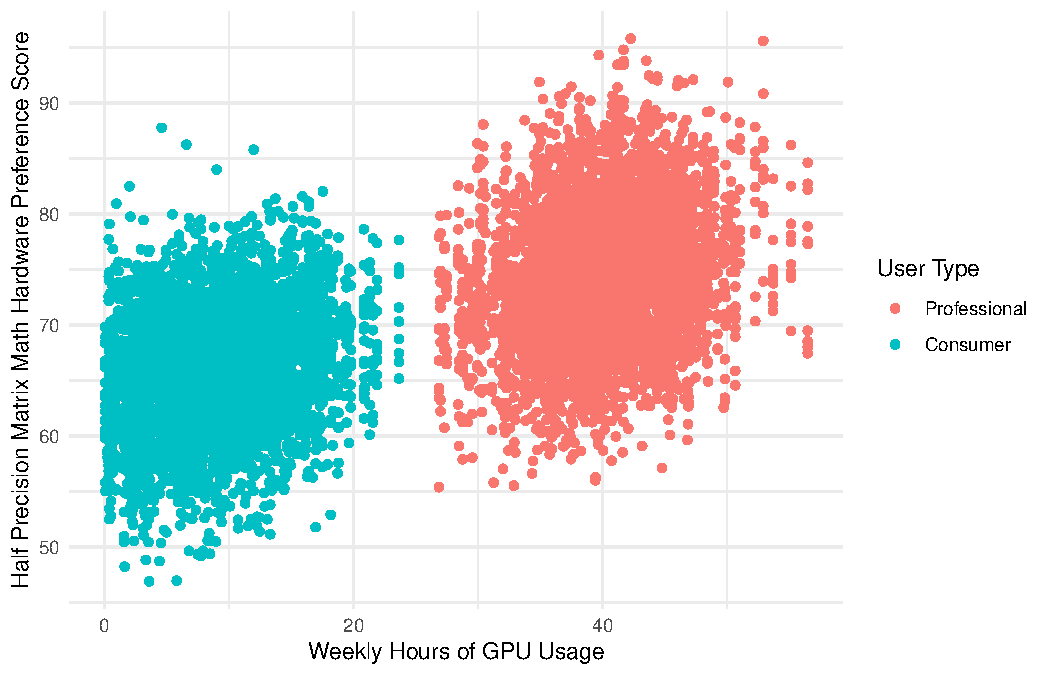
\includegraphics[width=0.6\linewidth,]{Assignment1_files/figure-latex/unnamed-chunk-8-1} 

}

\caption{Weekly Hours of GPU Usage vs Half Precision Hardware Preference Score}\label{fig:unnamed-chunk-8}
\end{figure}

From the scatter plot of \texttt{Weekly\ Hours\ of\ GPU\ Usage} versus
\texttt{Half\ Precision\ Matrix\ Math\ Hardware\ Preference\ Score}, we
see that both distributions are also approximately Gaussian; however the
consumer distribution is not exactly Gaussian as weekly hours of GPU
usage must be greater than 0. Additionally, the Professional category of
users has a generally higher preference for half precision matrix math
hardware. It appears that the difference between the two user groups is
just a shift up/down, i.e., consumers appear to have been shifted down
by some constant. The spread between the distributions appear to be
similar in general.

There are additional plots in the appendix that depict the scatterplots
above, but separated by the corresponding GPU type and primary
interaction with their GPU. From the additional scatter plots, we can
see that there are fairly noticeable changes in the slope of the scatter
plot

\textbf{Note about simulation:} The data was simulated specifically
using the R language with base R packages and the R library
\texttt{extraDistr} for sampling from a categorical distribution
{[}20{]}.

\hypertarget{methods}{%
\subsection{Methods}\label{methods}}

First from our plots, we see that in some cases, there is a pretty clear
visual distinction between the preferences of GPU hardware capabilities
of professional versus consumers. In particular, ray-tracing hardware
seems to have a very clear difference. This indicates that potentially
we will need to employ a model that considers this, i.e., a mixed
effects model. At a high level, a mixed effects model is just one that
allows for more granularity to the model coefficients by allowing for
the coefficient of each variable to be adjusted based on some other
categorical variable or for the intercept to be adjusted based some
other categorical variable. While other flexible models exist, a mixed
effects model is much more interpretable (consider a neural network with
thousands of parameters versus a mixed effects model with a few). So our
modelling approach was a hierarchical one as we believe that the
preference scores are affected by an overarching variable, i.e., the
user type. To gather evidence of this hierarchical nature, we calculated
a 95\% confidence interval for the difference in means (using unequal
variances) in independent samples. So we made sure it is appropriate to
do so, i.e., checked for normality (if the data conforms to the bell
shaped normal distribution) using QQ-plots, and we employed the F-test
for equal variances.

As a note about investigating normality, we will not use normality
tests. This is because the standard Shapiro-Wilk test is too sensitive
on large sample sizes, e.g., over 5000 (which is the sample size limit
in R and we exceed that). So even if we have small deviations from
normality, we will get evidence of it even if the tests at this sample
size, e.g, T-tests, are robust to such deviations. {[}11{]} The
Kolmogorov-Smirnov test is another common one, but that test has low
power and we must estimate our distributional parameters from data.
Instead QQ-plots are preferred due to easy of interpretation at large
sample sizes. {[}11{]}

Then for the F-test for equal variances, we used a two tailed F-test
using the hypotheses:

\[
\begin{aligned}
\text{H}_0&: \sigma^2_\text{Professional GPU User} = \sigma^2_\text{Consumer GPU User}\\
\text{H}_a&: \sigma^2_\text{Professional GPU User} \neq \sigma^2_\text{Consumer GPU User}
\end{aligned}
\]

We use the following test statistic:

\[
F = \frac{\sigma^2_\text{Professional GPU User}}{\sigma^2_\text{Consumer GPU User}}
\]

Note that the \(F\) test statistic above follows an F distribution with
\(n-1\) and \(m-1\) degrees of freedom under the null hypothesis. Also
since the number of samples between user types are unlikely to be equal,
we will randomly sample 1000 samples from each subgroup.

Due to the small p-value then we have evidence that the variances of
distributions among the two types of GPU users is not equal, which
motivated us to use a confidence interval with unequal variances.

Our confidence interval will compare the difference in means of the
distributions of the Professional GPU User scores to those of Consumer
GPU User scores. We will do this three times, with one for each
category, we are not performing multiple testing and do not need
correction (e.g., Bonferroni correction). We opt for a confidence
interval over a hypothesis test because we wish to explore the effect
size of the difference in the means rather than the point estimate
exactly. If the confidence interval (CI) does not contain 0, then we can
also conclude that there's a statistically significant difference in the
means. We will compute the confidence interval as {[}14{]}:

\[
\begin{aligned}
(\hat{\mu}_{\text{professional}} - \hat{\mu}_{\text{consumer}}) &\pm t^* \sqrt{\frac{s^2_{\text{professional}}}{n_{\text{professional}}} + \frac{s^2_{\text{consumer}}}{n_{\text{consumer}}}} \\
t^* &= t_{(\alpha/0.2, ~ df)} \\
df &= n_{\text{professional}} + n_{\text{consumer}} - 2
\end{aligned}
\]

Our analysis for our results consists of mixed effects models that
separately measure the preference for traditional GPU cores,
ray-tracing, and half-precision matrix math hardware. In particular, we
have three models using the same model specification but different
response variables. So we have a model for each one of the preferences
for traditional GPU cores, ray-tracing, and half-precision matrix math
hardware. We construct these three models separately because we want to
be able to examine each response variable, i.e., the preferences of the
three categories of hardware separately. This can allow us to see if we
get different effect size estimates for the same covariates with a
different response variable. Recall that an effect size is simply the
coefficient of a model for some variable, which is generally written as
\(\beta_{k}\) for the \(k^{th}\) coefficient/variable. We'll
specifically model the response variable using a mixed effects model,
where the response follows a normal distribution. So precisely, we are
using a linear mixed effects model. We make this modelling choice as the
data is continuous and does not appear to be constrained (no need for a
distribution like a truncated normal), and from the graphs above, they
appear to be approximately normally distributed. Additionally, we add a
so-called random effect due to the user type, which, as discussed above,
is motivated from the observation that scores are separated by user
types. In particular, we add a random intercept, meaning the intercept
of the model is adjusted for each user type. We also add random slopes
(adjust the coefficients for each variable by the user type) for the
\texttt{Primary\ GPU\ Interaction} and \texttt{Type\ of\ GPU} variables
because as discussed in the survey creation, we believe that different
user types would consider the same GPU interaction and GPU type
differently, meaning we'd need to adjust the coefficients based on user
type. For our primary model we do not add a random slope to the
\texttt{Estimated\ Hours\ of\ Daily\ GPU\ Usage} variable because
visually it appears that coefficient for that variable is constant
across user types. However we investigate this further with a more
complex model and present the results in the results section. We define
our primary model as follows:

\[
\begin{aligned}
y_i &\sim N(\mu_i, \sigma^2) \\
\mu_i = \beta_0 + (\beta_1 + U_{1j})\cdot\text{Primary GPU Interaction}& + (\beta_2 + U_{2j})\cdot\text{Type of GPU}_i \\+~ \beta_3~ \cdot &~\text{Estimated Hours of Daily GPU Usage}_i + U_{3j} \\
U_{1} &\sim N(0, \tau_1) \\
U_2 &\sim N(0, \tau_2) \\
U_{3} &\sim N(0, \tau_{3})
\end{aligned}
\]

Note that above, \(\beta_0\) is the intercept, and \(U_1j\) is the
random slope for the \texttt{Primary\ GPU\ Interaction} for the
\(j^{th}\) user group, \(U_2j\) is the random slope for the
\texttt{Type\ of\ GPU} for the \(j^{th}\) user group, and \(U_{3j}\) is
the random intercept for the \(j^{th}\) user group. Then
\(U_1 \sim N(0, \tau_1)\), \(U_2 \sim N(0, \tau_2)\), and
\(U_3 \sim N(0, \tau_3)\), meaning that these random effects are
described by a normal distribution centered around 0 with some standard
deviations. The random effects are from distributions from centered
around 0 because they may not have an effect for some group, and are
given independent standard deviations as this allows for more
granularity, e.g., the user type may affect the
\texttt{Primary\ GPU\ Interaction} differently than how it affects
\texttt{Type\ of\ GPU}.

As mentioned above we also investigate if the
\texttt{Estimated\ Hours\ of\ Daily\ GPU\ Usage} variable also needs a
random slope for the user type, i.e, if the user type affects
\texttt{Estimated\ Hours\ of\ Daily\ GPU\ Usage} coefficient differently
by user type. In this case, we use the same variable but with one
additional random slope:

\[
\begin{aligned}
y_i &\sim N(\mu_i, \sigma^2) \\
\mu_i = \beta_0 + (\beta_1 + U_{1j})\cdot \text{Primary GPU Interaction} &+ (\beta_2 + U_{2j})\cdot\text{Type of GPU}_i \\~+ ~(\beta_3 + U_{4j}) ~ &\cdot ~\text{Estimated Hours of Daily GPU Usage}_i + U_{3j} \\
U_{1} &\sim N(0, \tau_1) \\
U_2 &\sim N(0, \tau_2) \\
U_{3} &\sim N(0, \tau_{3}) \\
U_{4} &\sim N(0, \tau_{4})
\end{aligned}
\]

For brevity sake, we will not discuss the model in detail again. The
singular addition to this model is \(U_{4j}\), which is the random slope
that enables a different coefficient for
\texttt{Estimated\ Hours\ of\ Daily\ GPU\ Usage} based on user type.
\(U_4\) is distributed by a \(N(0, \tau_4)\) distribution for the same
reasons above.

Recall that we chose a linear mixed effects model over other flexible
choices like neural networks because linear mixed effects models are
relatively easy to interpret. However, adding this random slope makes
the model more complicated to interpret, so we will use a
likelihood-ratio test to determine if it is worth adding this extra
complexity. To do so, we will use the R package \texttt{lmtest}
{[}16{]}.

The likelihood-ratio test examines if the data has as higher likelihood
under our more complex model, i.e., if the model is essentially a better
fit. If the more complex model is significantly a better fit (has a
significantly higher likelihood), then we would choose the more complex
model. So the associated hypotheses are:

\[
\begin{aligned}
H_{0}&: \text{The simpler model is better} \\
H_{a}&: \text{The more complex model is better}
\end{aligned}
\]

So if we have a small p-value from the resulting test, then we have
evidence that the more complex model is better. We will opt to not show
the derivations of the test statistic as it is rather complex and is out
of the scope of this paper. For clarity, the test statistic we use is:

\[
-2 \log(\frac{\mathcal{L}_{\text{simple model}}(\hat{\theta}_{\text{simple model}}\mid x)}{\mathcal{L}_{\text{complex model}}(\hat{\theta}_{\text{complex model}} \mid x)})
\]

Note that \(\mathcal{L}(\hat{\theta} \mid x)\) is the log-likelihood
function provided data \(x\) and maximum likelihood estimated parameters
\(\hat{\theta}\).

Finally note that all of these models are fit using the R package
\texttt{lmer} {[}15{]}, and model specification as code is available in
the results section. All tables for results and in the rest of this
paper were prepared using the R package \texttt{knitr} {[}17{]}. With
our final models, we will present the coefficients, and interpret them
to analyze the effects of our covariates on our three hardware category
preference scores.

\hypertarget{results}{%
\subsection{Results}\label{results}}

First, we will examine the QQ-plots of all three preference score
categories, where each plot contains the QQ-plot for both consumer and
professional groups. This as discussed in the methods section will
examine if our data has worrying deviations from normality.

\begin{figure}

{\centering 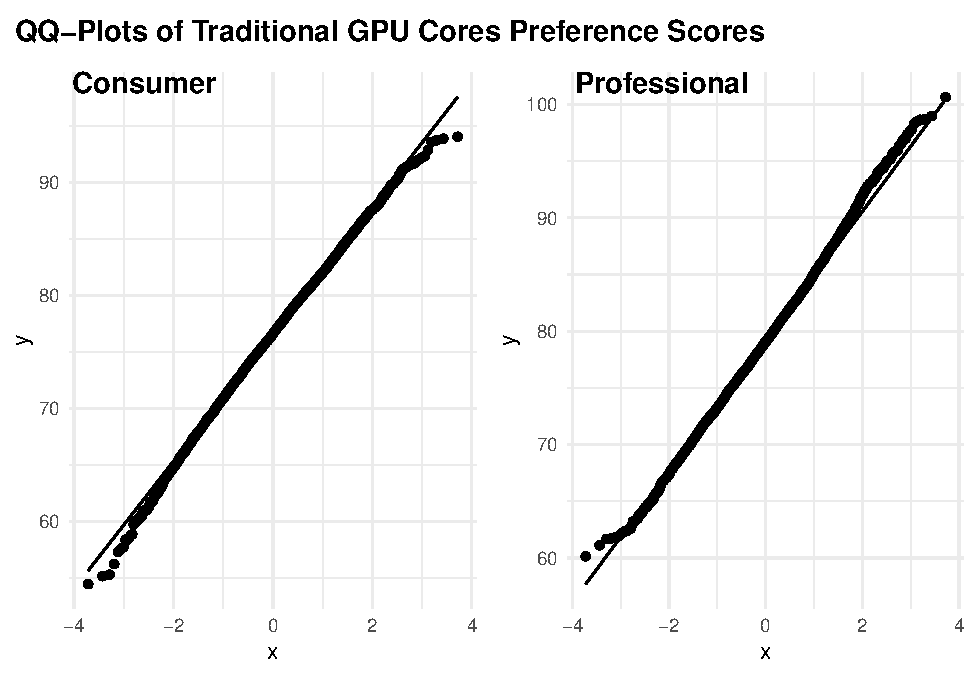
\includegraphics[width=0.6\linewidth,]{Assignment1_files/figure-latex/unnamed-chunk-11-1} 

}

\caption{QQ-plots for Traditional GPU Cores Preference Scores by User Type}\label{fig:unnamed-chunk-11}
\end{figure}

The above plot depicts the QQ-plots for Traditional GPU Cores preference
scores. In the consumer subplot, we see that the data mostly conforms to
a normal distribution, where there are some deviations in the tails. The
deviations in the upper tails are indicative of a very slightly lighter
than theoretical upper tail and a very slightly lighter heavier tail.
Additionally, it appears in the professional subplot, we see that the
data also mostly conforms to a normal distribution, but with some more
deviation in the upper tail. However, overall, these are small
deviations so we shouldn't be too worried about violating normality
assumptions.

\begin{figure}

{\centering 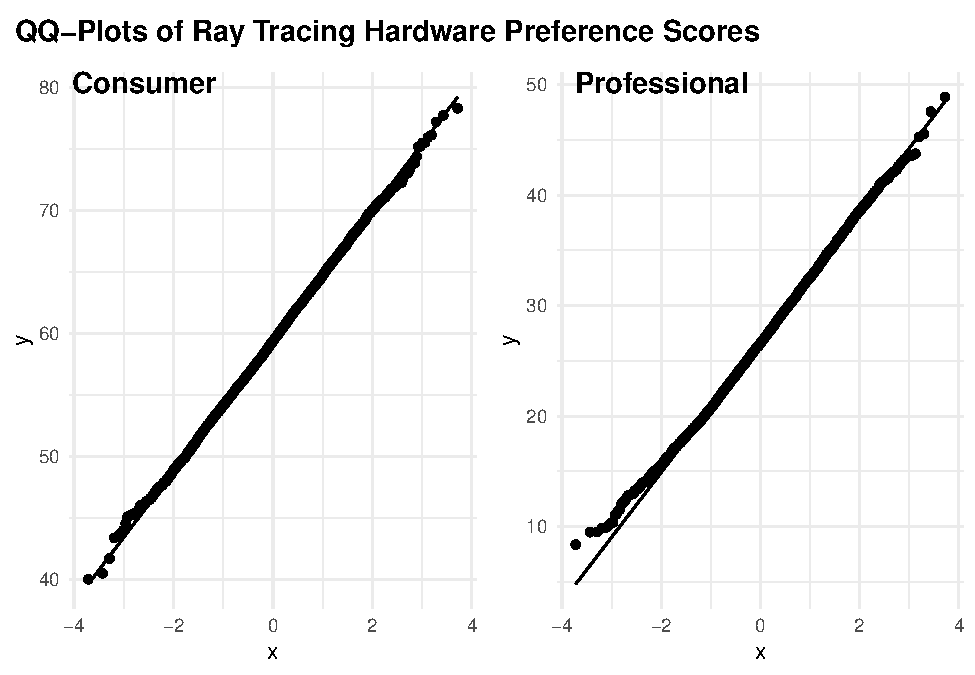
\includegraphics[width=0.6\linewidth,]{Assignment1_files/figure-latex/unnamed-chunk-12-1} 

}

\caption{QQ-plots for Ray Tracing Hardware Preference Scores by User Type}\label{fig:unnamed-chunk-12}
\end{figure}

The plot above depicts the QQ-plots for ray tracing hardware preference
scores by user category. In the consumer subplot, we see that there are
essentially no deviations from the QQ-plot line, i.e., we are not
concerned about violating normality assumptions. In the professional
subplot, we see that the only deviations from the QQ-plot line is in the
lower tail, where the deviation is potentially indicative of a lighter
than theoretical lower tail. Overall, we should not be very concerned
about violating normality assumptions since any deviations from QQ-plot
line are minor.

\begin{figure}

{\centering 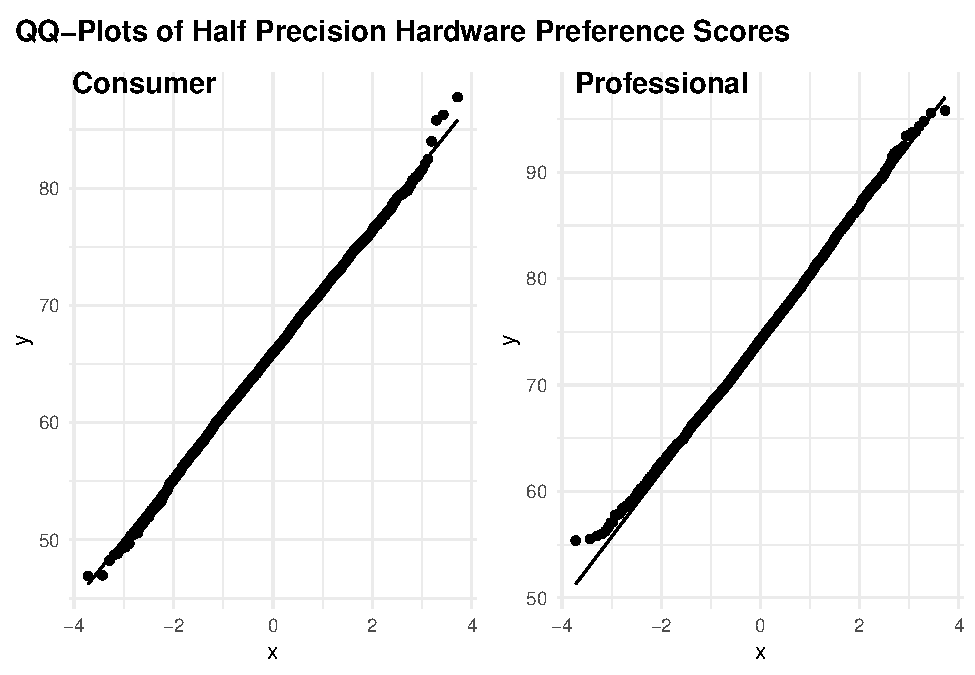
\includegraphics[width=0.6\linewidth,]{Assignment1_files/figure-latex/unnamed-chunk-13-1} 

}

\caption{QQ-plots for Half Precision Hardware Preference Scores by User Type}\label{fig:unnamed-chunk-13}
\end{figure}

The plot above depicts the QQ-plots for half precision matrix math
hardware preference scores by user category. In the consumer subplot, we
see that the only deviations from the QQ-plot line is in the upper tail,
where the deviation is indicative of a slightly heavier than theoretical
upper tail. In the professional subplot, we see a slight deviation from
the QQ-plot line in the lower tail, where the small deviation is
indicative of a slightly lighter than theoretical lower tail. Overall,
we should not be very concerned about violating normality assumptions
since any deviations from QQ-plot line are minor.

Then we examine the variances of the distributions by user type to see
if we have evidence of unequal variances. For that we conduct 3 F-tests
using the \texttt{var.test} command in R. We present a table with the
preference score category, the test statistic, numerator degrees of
freedom, denominator degrees of freedom, and the accompanying test
p-value:

\begin{longtable}[]{@{}
  >{\raggedright\arraybackslash}p{(\columnwidth - 8\tabcolsep) * \real{0.2000}}
  >{\raggedright\arraybackslash}p{(\columnwidth - 8\tabcolsep) * \real{0.2000}}
  >{\raggedright\arraybackslash}p{(\columnwidth - 8\tabcolsep) * \real{0.2000}}
  >{\raggedright\arraybackslash}p{(\columnwidth - 8\tabcolsep) * \real{0.2000}}
  >{\raggedright\arraybackslash}p{(\columnwidth - 8\tabcolsep) * \real{0.2000}}@{}}
\caption{F-test results for three hardware categories, comparing
professional vs consumer users}\tabularnewline
\toprule()
\begin{minipage}[b]{\linewidth}\raggedright
Score Category
\end{minipage} & \begin{minipage}[b]{\linewidth}\raggedright
F-statistic
\end{minipage} & \begin{minipage}[b]{\linewidth}\raggedright
Numerator DF
\end{minipage} & \begin{minipage}[b]{\linewidth}\raggedright
Denominator DF
\end{minipage} & \begin{minipage}[b]{\linewidth}\raggedright
P-value
\end{minipage} \\
\midrule()
\endfirsthead
\toprule()
\begin{minipage}[b]{\linewidth}\raggedright
Score Category
\end{minipage} & \begin{minipage}[b]{\linewidth}\raggedright
F-statistic
\end{minipage} & \begin{minipage}[b]{\linewidth}\raggedright
Numerator DF
\end{minipage} & \begin{minipage}[b]{\linewidth}\raggedright
Denominator DF
\end{minipage} & \begin{minipage}[b]{\linewidth}\raggedright
P-value
\end{minipage} \\
\midrule()
\endhead
Traditional GPU Cores & 1.113758 & 5069 & 4929 & 0.0001411 \\
Ray-tracing Hardware & 1.198882 & 5069 & 4929 &
\(1.511 \cdot 10^{-10}\) \\
Half Precision Hardware & 1.304594 & 5069 & 4929 & \textless{}
\(2.2 \cdot 10^{-16}\) \\
\bottomrule()
\end{longtable}

From the F-test results, we have extremely strong evidence in all three
hardware categories of different variances between the distributions of
professional and consumer users.

Since we feel comfortable with our normality assumption, i.e., our
distributions are all approximately normal, we compute a confidence
interval, using the R command \texttt{t.test}, for the differences in
means between the three score categories separately.

\begin{longtable}[]{@{}
  >{\raggedright\arraybackslash}p{(\columnwidth - 6\tabcolsep) * \real{0.2500}}
  >{\raggedright\arraybackslash}p{(\columnwidth - 6\tabcolsep) * \real{0.2500}}
  >{\raggedright\arraybackslash}p{(\columnwidth - 6\tabcolsep) * \real{0.2500}}
  >{\raggedright\arraybackslash}p{(\columnwidth - 6\tabcolsep) * \real{0.2500}}@{}}
\caption{Confidence Interval for Traditional GPU Cores, Comparing
Professional vs Consumer Users}\tabularnewline
\toprule()
\begin{minipage}[b]{\linewidth}\raggedright
Lower Bound of CI
\end{minipage} & \begin{minipage}[b]{\linewidth}\raggedright
Upper Bound of CI
\end{minipage} & \begin{minipage}[b]{\linewidth}\raggedright
Sample mean of Professional Users
\end{minipage} & \begin{minipage}[b]{\linewidth}\raggedright
Sample Mean of Consumer users
\end{minipage} \\
\midrule()
\endfirsthead
\toprule()
\begin{minipage}[b]{\linewidth}\raggedright
Lower Bound of CI
\end{minipage} & \begin{minipage}[b]{\linewidth}\raggedright
Upper Bound of CI
\end{minipage} & \begin{minipage}[b]{\linewidth}\raggedright
Sample mean of Professional Users
\end{minipage} & \begin{minipage}[b]{\linewidth}\raggedright
Sample Mean of Consumer users
\end{minipage} \\
\midrule()
\endhead
2.43740 & 2.89307 & 79.17382 & 76.50853 \\
\bottomrule()
\end{longtable}

From our confidence interval examining the means of the traditional GPU
cores preference scores of professionals and consumers, we find very
strong evidence of evidence that the difference of means is not equal to
0. While the difference is small, i.e., \(\approx 3\), the p-value is
less than \(2.2 \cdot 10^{-16}\), i.e., very strong evidence of a
difference in means. Thus, we conclude that it could be appropriate to
use a mixed effects model for modelling the preference scores of
traditional GPU cores.

\begin{longtable}[]{@{}
  >{\raggedright\arraybackslash}p{(\columnwidth - 6\tabcolsep) * \real{0.2500}}
  >{\raggedright\arraybackslash}p{(\columnwidth - 6\tabcolsep) * \real{0.2500}}
  >{\raggedright\arraybackslash}p{(\columnwidth - 6\tabcolsep) * \real{0.2500}}
  >{\raggedright\arraybackslash}p{(\columnwidth - 6\tabcolsep) * \real{0.2500}}@{}}
\caption{Confidence Interval for Ray Tracing Hardware, Comparing
Professional vs Consumer Users}\tabularnewline
\toprule()
\begin{minipage}[b]{\linewidth}\raggedright
Lower Bound of CI
\end{minipage} & \begin{minipage}[b]{\linewidth}\raggedright
Upper Bound of CI
\end{minipage} & \begin{minipage}[b]{\linewidth}\raggedright
Sample mean of Professional Users
\end{minipage} & \begin{minipage}[b]{\linewidth}\raggedright
Sample Mean of Consumer users
\end{minipage} \\
\midrule()
\endfirsthead
\toprule()
\begin{minipage}[b]{\linewidth}\raggedright
Lower Bound of CI
\end{minipage} & \begin{minipage}[b]{\linewidth}\raggedright
Upper Bound of CI
\end{minipage} & \begin{minipage}[b]{\linewidth}\raggedright
Sample mean of Professional Users
\end{minipage} & \begin{minipage}[b]{\linewidth}\raggedright
Sample Mean of Consumer users
\end{minipage} \\
\midrule()
\endhead
-32.91641 & -32.48230 & 26.70695 & 59.40630 \\
\bottomrule()
\end{longtable}

Then from our confidence interval examining the difference in means of
the ray tracing hardware preference scores of professionals and
consumers, we a relatively small range from (-32.92, -32.48) for the
true difference. The difference is very large, i.e., \(\approx -33\),
and shows very strong statistically significant evidence that the mean
preference score is different between professionals and consumers at the
95\% significance level as 0 is not in the interval. Thus, we gather
additional evidence that it is appropriate to use a mixed effects model
for modelling the preference scores of ray tracing hardware.

\begin{longtable}[]{@{}
  >{\raggedright\arraybackslash}p{(\columnwidth - 6\tabcolsep) * \real{0.2500}}
  >{\raggedright\arraybackslash}p{(\columnwidth - 6\tabcolsep) * \real{0.2500}}
  >{\raggedright\arraybackslash}p{(\columnwidth - 6\tabcolsep) * \real{0.2500}}
  >{\raggedright\arraybackslash}p{(\columnwidth - 6\tabcolsep) * \real{0.2500}}@{}}
\caption{Confidence Interval for Half Precision Hardware, Comparing
Professional vs Consumer Users}\tabularnewline
\toprule()
\begin{minipage}[b]{\linewidth}\raggedright
Lower Bound of CI
\end{minipage} & \begin{minipage}[b]{\linewidth}\raggedright
Upper Bound of CI
\end{minipage} & \begin{minipage}[b]{\linewidth}\raggedright
Sample mean of Professional Users
\end{minipage} & \begin{minipage}[b]{\linewidth}\raggedright
Sample Mean of Consumer users
\end{minipage} \\
\midrule()
\endfirsthead
\toprule()
\begin{minipage}[b]{\linewidth}\raggedright
Lower Bound of CI
\end{minipage} & \begin{minipage}[b]{\linewidth}\raggedright
Upper Bound of CI
\end{minipage} & \begin{minipage}[b]{\linewidth}\raggedright
Sample mean of Professional Users
\end{minipage} & \begin{minipage}[b]{\linewidth}\raggedright
Sample Mean of Consumer users
\end{minipage} \\
\midrule()
\endhead
8.143725 & 8.592351 & 74.32353 & 65.95549 \\
\bottomrule()
\end{longtable}

Finally from our confidence interval of the difference in means of the
half precision matrix math hardware preference scores of professionals
and consumers, we find a relatively small range, i.e., 8.14 to 8.59. But
the difference is also comparably large (compared to that of traditional
GPU cores), i.e., \(\approx 8\), and shows very strong statistically
significant evidence that the mean preference score is different between
professionals and consumers at the 95\% significance level as 0 is not
in the interval. Thus, we conclude that it could also be appropriate to
use a mixed effects model for modelling the preference scores of half
precision matrix math hardware.

Since we are comfortable with our normality assumption and because the
means of the distributions by user group are significantly different,
meaning that we proceed with constructing a mixed effects model. The
model architecture follows that as described in the methods section, and
primarily our investigation here concerns if we should add a random
slope to the weekly hours of GPU use variable for the user types. As
mentioned in the methods section, we performed likelihood ratio tests
for each of the three hardware categories, comparing the complex model
with the extra random slope to the model without the random slope
(reduced model). We find in all three cases that the complex model is
not needed, i.e., the complex model does not provide a better fit.

For reference we fit the following models using the R package
\texttt{lmer} {[}15{]} and all likelihood ratio tests were conducted
using R package \texttt{lmtest} {[}16{]}:

\begin{itemize}
\tightlist
\item
  Traditional GPU Cores Preference Scores:

  \begin{itemize}
  \tightlist
  \item
    Reduced model:
    \texttt{model.tradGPUCores\ \textless{}-\ lmer(simulations.tradGPUCores\ \textasciitilde{}\ weeklyHours\ +\ primaryInteraction\ +\ GPUType\ +\ (1\ +\ primaryInteraction\ +\ GPUType\ \textbar{}\ user),\ data\ =\ sim.survey)}
  \item
    Complex model:
    \texttt{model.extra.tradGPUCores\ \textless{}-\ lmer(simulations.tradGPUCores\ \textasciitilde{}\ weeklyHours\ +\ primaryInteraction\ +\ GPUType\ +\ (1\ +\ primaryInteraction\ +\ GPUType\ +\ weeklyHours\ \textbar{}\ user),\ data\ =\ sim.survey)}
  \end{itemize}
\item
  Ray Tracking Hardware Preference Scores:

  \begin{itemize}
  \tightlist
  \item
    Reduced model:
    \texttt{model.rayTraced\ \textless{}-\ lmer(simulations.rayTraced\ \textasciitilde{}\ weeklyHours\ +\ primaryInteraction\ +\ GPUType\ +\ (1\ +\ primaryInteraction\ +\ GPUType\ \textbar{}\ user),\ data\ =\ sim.survey)}
  \item
    Complex model:
    \texttt{model.extra.rayTraced\ \textless{}-\ lmer(simulations.rayTraced\ \textasciitilde{}\ weeklyHours\ +\ primaryInteraction\ +\ GPUType\ +\ (1\ +\ primaryInteraction\ +\ GPUType\ +\ weeklyHours\ \textbar{}\ user),\ data\ =\ sim.survey)}
  \end{itemize}
\item
  Half Precision Matrix Math Hardware Preference Scores:

  \begin{itemize}
  \tightlist
  \item
    Reduced model:
    \texttt{model.halfPrecision\ \textless{}-\ lmer(simulations.halfPrecision\ \textasciitilde{}\ weeklyHours\ +\ primaryInteraction\ +\ GPUType\ +\ (1\ +\ primaryInteraction\ +\ GPUType\ \textbar{}\ user),\ data\ =\ sim.survey)}
  \item
    Complex model:
    \texttt{model.extra.halfPrecision\ \textless{}-\ lmer(simulations.halfPrecision\ \textasciitilde{}\ weeklyHours\ +\ primaryInteraction\ +\ GPUType\ +\ (1\ +\ primaryInteraction\ +\ GPUType\ +\ weeklyHours\ \textbar{}\ user),\ data\ =\ sim.survey)}
  \end{itemize}
\end{itemize}

\begin{longtable}[]{@{}rrrrr@{}}
\caption{Traditional GPU Cores Models Likelihood Ratio
Test}\tabularnewline
\toprule()
\#Df & LogLik & Df & Chisq & Pr(\textgreater Chisq) \\
\midrule()
\endfirsthead
\toprule()
\#Df & LogLik & Df & Chisq & Pr(\textgreater Chisq) \\
\midrule()
\endhead
15 & -30286.86 & NA & NA & NA \\
11 & -30285.96 & -4 & 1.782022 & 0.7757699 \\
\bottomrule()
\end{longtable}

The table above is the result of the likelihood ratio test between the
complex model and the reduced model for the traditional GPU cores
preference scores. As shown, the p-value is 0.775, so we have no
evidence that the complex model for the traditional GPU cores preference
scores being better. For conducting the likelihood ratio test, we use
the following R function call
\texttt{lmtest::lrtest(model.extra.tradGPUCores,\ model.tradGPUCores)}.

\begin{longtable}[]{@{}rrrrr@{}}
\caption{Half Precision Hardware Models Likelihood Ratio
Test}\tabularnewline
\toprule()
\#Df & LogLik & Df & Chisq & Pr(\textgreater Chisq) \\
\midrule()
\endfirsthead
\toprule()
\#Df & LogLik & Df & Chisq & Pr(\textgreater Chisq) \\
\midrule()
\endhead
15 & -30312.59 & NA & NA & NA \\
11 & -30309.00 & -4 & 7.182054 & 0.1265746 \\
\bottomrule()
\end{longtable}

The table above is the result of the likelihood ratio test between the
complex model and the reduced model for the half precision hardware
preference scores. As shown, the p-value is 0.126, so we have very
little evidence that the complex model for the traditional GPU cores
preference scores being better, which is insufficient to conclude that
the complex model is necessary even at the 0.1 significance level. For
conducting the likelihood ratio test, we use the following R function
call
\texttt{lmtest::lrtest(model.extra.halfPrecision,\ model.halfPrecision)}.

\begin{longtable}[]{@{}rrrrr@{}}
\caption{Ray Tracing Hardware Models Likelihood Ratio
Test}\tabularnewline
\toprule()
\#Df & LogLik & Df & Chisq & Pr(\textgreater Chisq) \\
\midrule()
\endfirsthead
\toprule()
\#Df & LogLik & Df & Chisq & Pr(\textgreater Chisq) \\
\midrule()
\endhead
15 & -30268.60 & NA & NA & NA \\
11 & -30268.83 & -4 & 0.4514466 & 0.9780523 \\
\bottomrule()
\end{longtable}

The table above is the result of the likelihood ratio test between the
complex model and the reduced model for the ray tracing hardware
preference scores. As shown, the p-value is 0.978, so we have
essentially no evidence that the complex model for the traditional GPU
cores preference scores being better. For conducting the likelihood
ratio test, we use the following R function call
\texttt{lmtest::lrtest(model.extra.rayTraced,\ model.rayTraced)}.

To summarize, our final models are the reduced complexity models as
concluded from the likelihood ratio test. We present the following
coefficients for the models. We will discuss the results comparatively
for each model by user type because we want to examine the trends
between GPU user groups. Note that for each of these tables, the
coefficients (effect sizes) for the professional users are presented in
the first row with consumers presented in the second row. First we will
examine the coefficients for the traditional GPU cores preference score
model coefficients:

\begin{longtable}[]{@{}
  >{\raggedright\arraybackslash}p{(\columnwidth - 8\tabcolsep) * \real{0.0417}}
  >{\raggedleft\arraybackslash}p{(\columnwidth - 8\tabcolsep) * \real{0.1389}}
  >{\raggedleft\arraybackslash}p{(\columnwidth - 8\tabcolsep) * \real{0.3611}}
  >{\raggedleft\arraybackslash}p{(\columnwidth - 8\tabcolsep) * \real{0.3333}}
  >{\raggedleft\arraybackslash}p{(\columnwidth - 8\tabcolsep) * \real{0.1250}}@{}}
\toprule()
\begin{minipage}[b]{\linewidth}\raggedright
\end{minipage} & \begin{minipage}[b]{\linewidth}\raggedleft
Intercept
\end{minipage} & \begin{minipage}[b]{\linewidth}\raggedleft
Weekly Hours of GPU Usage
\end{minipage} & \begin{minipage}[b]{\linewidth}\raggedleft
Primary GPU Interaction
\end{minipage} & \begin{minipage}[b]{\linewidth}\raggedleft
GPU Type
\end{minipage} \\
\midrule()
\endhead
0 & 60.30327 & 0.2471844 & 3.983912 & 1.865748 \\
1 & 59.99129 & 0.2471844 & 3.876773 & 1.103765 \\
\bottomrule()
\end{longtable}

From there, we see that it seems there is a difference between the
coefficient estimate for the GPU Type between professionals and
consumers. As in, GPU type contributes to traditional GPU cores
preference scores almost twice as much in professionals (first row) when
compared to consumers. In other words, professionals should expect to
see around a 2 point increase for each GPU level they go up in (moving
to more expensive/performant GPU categories), while consumers should
only expect to see about a 1 point increase in their traditional GPU
cores preference scores. All of the other effect sizes are extremely
similar between professionals and consumers, e.g., the baseline
preference score (intercept) for both is about 60. Additionally, our
model estimates that for each hour extra of weekly GPU usage, both
consumers and professionals will expect to see an \(\approx 0.25\)
increase in preference for traditional GPU cores. Finally, for each
increase in the ``level'' of primary GPU interaction (moving to less
abstracted interactions with GPUs), both consumers and professionals
should expect to see about a 4 point increase in their preferences for
traditional GPU cores.

Then we examine the ray tracing hardware preference score model
coefficients:

\begin{longtable}[]{@{}
  >{\raggedright\arraybackslash}p{(\columnwidth - 8\tabcolsep) * \real{0.0411}}
  >{\raggedleft\arraybackslash}p{(\columnwidth - 8\tabcolsep) * \real{0.1370}}
  >{\raggedleft\arraybackslash}p{(\columnwidth - 8\tabcolsep) * \real{0.3562}}
  >{\raggedleft\arraybackslash}p{(\columnwidth - 8\tabcolsep) * \real{0.3288}}
  >{\raggedleft\arraybackslash}p{(\columnwidth - 8\tabcolsep) * \real{0.1370}}@{}}
\toprule()
\begin{minipage}[b]{\linewidth}\raggedright
\end{minipage} & \begin{minipage}[b]{\linewidth}\raggedleft
Intercept
\end{minipage} & \begin{minipage}[b]{\linewidth}\raggedleft
Weekly Hours of GPU Usage
\end{minipage} & \begin{minipage}[b]{\linewidth}\raggedleft
Primary GPU Interaction
\end{minipage} & \begin{minipage}[b]{\linewidth}\raggedleft
GPU Type
\end{minipage} \\
\midrule()
\endhead
0 & 9.988032 & 0.2441839 & 4.110996 & 0.4393086 \\
1 & 50.369219 & 0.2441839 & 1.922117 & 0.4716711 \\
\bottomrule()
\end{longtable}

Immediately, we notice that the baseline preferences for ray tracing
hardware is extremely different between professionals and consumers. Our
models tells us to expect about a 10 for a baseline preference score for
professionals while we should expect about a 50 for consumers. Another
difference of note is that the coefficeint estimate for primary GPU
interaction is almost double in professionals when compared to consumers
(\(\approx 4\) vs \(\approx 2\)), i.e., professionals should expect to
see about a 4 point increase in ray tracing hardware preference scores
if they increase their primary GPU interaction to the next level (make
their activities less abstracted away from the GPU), while consumers
should only expect to see an increase of about 2. Finally both weekly
hours of GPU usage and GPU type appear to be similar between
professionals and consumers. Both professionals and consumers should
expect to see an increase of \(\approx 0.24\) in their ray tracing
hardware scores for each additional hour of weekly GPU usage, while
increasing the GPU quality they use by one level should expect to see an
\(\approx 0.45\) increase to ray tracing hardware preference scores.

Finally we examine the half precision matrix math preference score model
coefficients:

\begin{longtable}[]{@{}
  >{\raggedright\arraybackslash}p{(\columnwidth - 8\tabcolsep) * \real{0.0417}}
  >{\raggedleft\arraybackslash}p{(\columnwidth - 8\tabcolsep) * \real{0.1389}}
  >{\raggedleft\arraybackslash}p{(\columnwidth - 8\tabcolsep) * \real{0.3611}}
  >{\raggedleft\arraybackslash}p{(\columnwidth - 8\tabcolsep) * \real{0.3333}}
  >{\raggedleft\arraybackslash}p{(\columnwidth - 8\tabcolsep) * \real{0.1250}}@{}}
\toprule()
\begin{minipage}[b]{\linewidth}\raggedright
\end{minipage} & \begin{minipage}[b]{\linewidth}\raggedleft
Intercept
\end{minipage} & \begin{minipage}[b]{\linewidth}\raggedleft
Weekly Hours of GPU Usage
\end{minipage} & \begin{minipage}[b]{\linewidth}\raggedleft
Primary GPU Interaction
\end{minipage} & \begin{minipage}[b]{\linewidth}\raggedleft
GPU Type
\end{minipage} \\
\midrule()
\endhead
0 & 54.38693 & 0.2591262 & 4.139309 & 2.091543 \\
1 & 54.38693 & 0.2591262 & 2.116416 & 1.037357 \\
\bottomrule()
\end{longtable}

We notice that the baseline preference and the coefficient for weekly
hours of GPU usage between professionals and consumers is the same for
half precision hardware. So we expect that both user types have a
baseline of about 54 points. While we also expect that for both user
types, an hour increase in weekly GPU usage results in a
\(\approx 0.26\) increase in half precision hardware preference score.
However, we also see that the coefficient for primary GPU interaction
for professionals is almost double that of consumers, i.e., for each
increase in primary GPU interaction level (moving to activities less
abstracted away from the GPU), we would expect to see an increase in 4
points for half precision hardware for professionals while consumers
should only expect about 2. Then similarly, for GPU type, moving to the
next higher quality GPU level, professionals should expect to see about
a 2 point increase in half precision hardware scores while consumers
should only expect to see about 1.

So overall, there are some interesting trends. Professionals and
consumers appear to have about the same baseline preference for both
traditional GPU cores and half precision hardware, but they greatly
differ when it comes to ray tracing hardware with consumers greatly
favouring ray tracing hardware relative to professionals. Generally,
across hardware categories, the baseline preference for all hardware
categories are fairly neutral (around 50), but it appears that
professionals simply do not prefer ray tracing hardware as a baseline
perhaps indicative of the lack of application in their domain {[}2{]}.
Additionally, we see that in the cases of ray tracing hardware and half
precision hardware, changing a professional's primary GPU interaction
will be much more impactful than doing the same with a consumer. This
observation also occurs with GPU types for traditional GPU cores and
half precision hardware. So it appears that professionals are more
easily influenced into potentially liking a hardware category should
they change up their hardware (a more powerful GPU) or their use cases
when compared to a consumer, which may be indicative that professionals
whose work requires a certain use case or quality of GPU prefer the
hardware that their use case, GPU type combination entails. Finally,
despite different opinions on different hardware categories, the hours a
user uses their GPU seems to affect preference scores equally across
hardware categories, suggesting that a particular hardware feature won't
affect the preferences of a user more strongly over other hardware
features.

\hypertarget{bibliography}{%
\subsection{Bibliography}\label{bibliography}}

\begin{enumerate}
\def\labelenumi{\arabic{enumi}.}
\tightlist
\item
  Evanson, Nick. ``Explainer: What Are Tensor Cores?'' TechSpot,
  TechSpot, 27 July 2020,
  \url{https://www.techspot.com/article/2049-what-are-tensor-cores}.
\item
  Ravenscraft, Eric. ``Should Anyone Actually Care about Ray Tracing?''
  Wired, Conde Nast, 3 Mar.~2021,
  \url{https://www.wired.com/story/should-anyone-actually-care-about-ray-tracing}.
\item
  Caulfield, Brian. ``CPU vs GPU: What's the Difference?'' NVIDIA Blog,
  23 June 2022,
  \url{https://blogs.nvidia.com/blog/2009/12/16/whats-the-difference-between-a-cpu-and-a-gpu}.
\item
  ``GPU Processing Unit (GPU) Market'' Allied Market Research,
  \url{https://bit.ly/3BLAyWQ}.
\item
  ``AMD Reports First Quarter 2022 Financial Results.'' Advanced Micro
  Devices, Inc., 3 May 2022,
  \url{https://ir.amd.com/news-events/press-releases/detail/1062/amd-reports-first-quarter-2022-financial-results}.
\item
  ``Nvidia Announces Financial Results for First Quarter Fiscal 2023.''
  NVIDIA Newsroom, 20 Sept.~2022,
  \url{https://nvidianews.nvidia.com/news/nvidia-announces-financial-results-for-first-quarter-fiscal-2023}.
\item
  Pandey, Mohit, et al.~``The Transformational Role of GPU Computing and
  Deep Learning in Drug Discovery.'' Nature News, Nature Publishing
  Group, 23 Mar.~2022,
  \url{https://www.nature.com/articles/s42256-022-00463-x}.
\item
  CSLab Support,
  \url{https://support.cs.toronto.edu/systems/linuxgpu.html}.
\item
  ``Games Industry Data and Analysis.'' Video Game Insights,
  \url{https://vginsights.com/insights/article/report-steam-games-market-size-likely-to-decline-in-2022-after-reaching-6-6bn-in-2021}.
\item
  Combs, Veronica, et al.~``8 Hours and 27 Minutes. That's How Long the
  Average Gamer Plays Each Week.'' TechRepublic, 22 Sept.~2022,
  \url{https://www.techrepublic.com/article/8-hours-and-27-minutes-thats-how-long-the-average-gamer-plays-each-week/}.
\item
  Ghasemi, Asghar, and Saleh Zahediasl. ``Normality tests for
  statistical analysis: a guide for non-statisticians.'' International
  journal of endocrinology and metabolism vol.~10,2 (2012): 486-9.
  \url{doi:10.5812/ijem.3505}
\item
  ``Best Buy Midrange GPU.'' BestBuy.com,
  \url{https://www.bestbuy.com/site/shop/best-mid-range-graphics-card}.
\item
  ``Best Buy High End GPU.'' BestBuy.com,
  \url{https://www.bestbuy.com/site/shop/high-end-graphics-cards}.
\item
  ``Difference in Means.'' Calcworkshop, 10 Oct.~2020,
  \url{https://calcworkshop.com/confidence-interval/difference-in-means/}.
\item
  Bates, D., M. Mächler, B. Bolker, and S. Walker. ``Fitting Linear
  Mixed-Effects Models Using Lme4''. Journal of Statistical Software,
  vol.~67, no. 1, Oct.~2015, pp.~1-48, \url{doi:10.18637/jss.v067.i01}.
\item
  ``Testing Linear Regression Models {[}R Package Lmtest Version
  0.9-40{]}.'' The Comprehensive R Archive Network, Comprehensive R
  Archive Network (CRAN), 21 Mar.~2022,
  \url{https://cran.r-project.org/web/packages/lmtest/index.html}.
\item
  Xie, Yihui. ``A General-Purpose Package for Dynamic Report Generation
  in R {[}R Package Knitr Version 1.40{]}.'' The Comprehensive R Archive
  Network, Comprehensive R Archive Network (CRAN), 24 Aug.~2022,
  \url{https://cran.r-project.org/web/packages/knitr/index.html}.
\item
  Martindale, Jon, et al.~``Nvidia RTX DLSS: Everything You Need to
  Know.'' Digital Trends, Digital Trends, 20 Sept.~2022,
  \url{https://www.digitaltrends.com/computing/everything-you-need-to-know-about-nvidias-rtx-dlss-technology/}.
\item
  ``Automatic Mixed Precision for Deep Learning.'' NVIDIA Developer, 18
  Feb.~2022,
  \url{https://developer.nvidia.com/automatic-mixed-precision}.
\item
  ``Package Extradistr.'' CRAN, Comprehensive R Archive Network (CRAN),
  \url{https://cran.r-project.org/web/packages/extraDistr/index.html}.
\end{enumerate}

\newpage

\hypertarget{appendix}{%
\subsection{Appendix}\label{appendix}}

Here is a glimpse of the data set simulated:

\begin{verbatim}
## Rows: 10,000
## Columns: 10
## $ user                      <int> 0, 0, 0, 0, 0, 0, 0, 0, 0, 0, 1, 1, 1, 1, 1,~
## $ primaryInteraction        <int> 1, 1, 1, 1, 1, 1, 1, 1, 1, 1, 3, 3, 3, 3, 3,~
## $ GPUType                   <int> 1, 1, 1, 1, 1, 1, 1, 1, 1, 1, 4, 4, 4, 4, 4,~
## $ weeklyHours               <dbl> 35.895067, 35.895067, 35.895067, 35.895067, ~
## $ ce.tradGPUCores           <dbl> 74.97377, 74.97377, 74.97377, 74.97377, 74.9~
## $ ce.rayTraced              <dbl> 23.47377, 23.47377, 23.47377, 23.47377, 23.4~
## $ ce.halfPrecision          <dbl> 69.97377, 69.97377, 69.97377, 69.97377, 69.9~
## $ simulations.tradGPUCores  <dbl> 71.57973, 77.84533, 71.45119, 72.30385, 78.8~
## $ simulations.rayTraced     <dbl> 33.68354, 26.54617, 25.58342, 20.99166, 25.9~
## $ simulations.halfPrecision <dbl> 76.18876, 79.88482, 66.74156, 74.80471, 62.8~
\end{verbatim}

\end{document}
